\documentclass{article}
\usepackage{indentfirst}
\usepackage{latexsym}
\usepackage{bm}
\usepackage{amsmath}
\usepackage{amssymb} 
\usepackage{tikz,mathpazo}
\usetikzlibrary{shapes.geometric, arrows}
\usepackage{flowchart}
\usepackage{subfigure}
\usepackage{hyperref}
\setlength{\parindent}{0em}


\title{Reconstruction based on Self-calibration in liquid scintillator detectors}  
\author{Dou Wei, Jianfeng Zhou}  
\date{\today}

\begin{document}

\maketitle
\abstract{}
\section{Introduction}
\subsection{Calibration of scintillator detector may bring extra challenges}
\begin{itemize}
\item {The advantages of scintillator detector} \\
1. Scintillator is a good candidate for neutrino observation for its better energy resolution and low energy threshold.\\
2. Calibration of a scintillation detector is a hard work.
\item {Why calibration so difficult} \\
1. The calibration source need high purity, which adds high difficulties to the mechanical process and demand high cost. \\
2. It is hard to fix calibration source in the detector, which may cause extra accident. \\
3. The structure of the calibration source may bring shadows which is different to the real situation, requiring more correction in simulation.
\item {Object is to reconstruct in no calibration detector} \\
1.  We try to reconstruct the vertex and unknown structures if we have plenty of data without calibration.\\
2.  If calibration is done, a cross check can be applied to reduce the error in measurement.\\
\end{itemize} 
\subsection{The importance of reconstruction}
\begin{itemize}
\item {Why reconstruction is so important?} \\
Reconstruction is necessary for:
     \begin{itemize}
	\item reduce the background
	\item raise the energy resolution
     \item identify the particle type
     \end{itemize}
\item {Who else has done that?} \\
1. Traditional reconstruction is a likelihood or divide detectors into many segment bins, careful calibration is needed \\
2. Recently Machine learning has broadly applied in background and particle type discrimination, physical process are omitted.\\
\item{Highlight of this paper and purpose of this paper} \\
1. This is the first series reconstruction without calibration in neutrino experiment. The main result provide a reconstruction of $\tau_d$ to future PID. We use software JSAP based on ROOT system and GEANT 4.\\
2. The sections are listed as following:
     \begin{itemize}
	\item Section 2 shows the how likelihood algorithm works. 
	\item Section 3 shows the simulation condition and reconstruction result. 
     \item Section 4 shows the conclusion and discussion.
     \end{itemize}
\end{itemize}

\section{Reconstruction Algorithm}
\subsection{Initial value of the reconstructed parameters}
1. A swift estimation using hit information to obtain a rough energy and vertex. 

    \begin{equation}
        \numberwithin{equation}{section}
        \vec{x}_{ini} = \frac{\sum_{i=1}^N n_i\vec{x}_i}{\sum_{i=1}^N n_i}
    \end{equation}

2. Decay Time constant dominate the time profile, assuming uncalibrated, energy dependent and particle dependent.

\subsection{`Conventional' likelihood algorithm}
	
\subsubsection{Traditional algorithm}

	We add a new uncalibrated parameter $\tau_d$ to traditional reconstruction algorithm, the former part only includes hit information and the latter includes time information readout by photo-sensors.
	\begin{equation}
		\numberwithin{equation}{section}
		\log \mathcal{L}\{\textbf{x},E,\tau_d, t_0;n_i,t_j\} = \log \mathcal{L}_{hit}\{\textbf{x},E;n_i\}+\log \mathcal{L}_{time}\{\textbf{x},\tau_d, t_0;t_j\}
	\end{equation}
	
	The likelihood is to calculate the probability of received photons by $i$-th PMT 

	\begin{equation}
	\numberwithin{equation}{section}
	p^*_i =  
		\begin{cases}
 		p_{i,hit}\{${\textbf x}$,E\} p_{i, time}\{${\textbf x}$, \tau_d, t_0\}& \text{$n_i > 0$ (Fired PMT)}\\
 		p_{i,hit}\{${\textbf x}$,E\} & \text{$n_i=0$ (Unfired PMT)}
		\end{cases}
	\end{equation}
	
	\begin{equation}
		\numberwithin{equation}{section}
		\log \mathcal{L}\{\textbf{x},E\} = \log \prod_{i} p^*_i = 	\sum_{i}\log p_{i,hit}\{\textbf{x},E\} +\sum_{i'}\log p_{i',time}\{\textbf{x},\tau_d, t_0\} 
	\end{equation}
	
	$i$ is the index of all PMTs and $i'$ only includes fired PMTs.   
\subsection{Based on hit information}
	\par The number of photon electrons received by PMT is approximately a Poisson process.
	
	\begin{equation}
	\numberwithin{equation}{section}
	p_i = \frac{\xi_i^{n_i}}{n_i!} \exp(-\xi_i)
	\end{equation}
	
	\par $\xi_i$ estimation needs to consider
	\begin{itemize}
		\item Initial energy $E$ and light yield $Y$
		\item The loss on propagation with attenuation length $L$
		\item The photo coverage $\Omega$ 
		\item Photo response with quantum efficiency $\eta_{QE}$
	\end{itemize}
	
	\par The expected photon on each PMT is also proportional to kinetic energy and light yield, therefore
	
	\begin{equation}
	\numberwithin{equation}{section}
	\xi_i = E\cdot Y\cdot \exp(-\frac{d_i({\textbf x})}{L(\lambda)}) \cdot \frac{\Omega_i({\textbf x})}{4\pi} \cdot\eta_{i,QE}(\lambda)
	\end{equation}

	\par Involving all the PMTs, the log likelihood is
	
	\begin{equation}
	\numberwithin{equation}{section}
	\log \mathcal{L}_{hit} = \sum_{i=1}^N \log p_{i,hit} \{{\textbf x},E;n_{i}\}
	\end{equation}
\subsection{Based on time information}
	\par The simplified lifetime of a scintillator photon can be generalized in 4 steps without scattering: 
	\begin{itemize}
	\item The particle at vertex $\textbf {x}$ begin the travel at $t_0$ like a point source.  
	\item The excited scintillator molecules emit photons with the randomly deexcite time $t_{j,p}$ satisfy time profile distribution $p(t)$, if finally received by $j$-th PMT.
	\item Photons flight to $j$-th PMT with flight time $t_{j,f}$ which is relative to the vertex.
	\item Photons deposit energy in PMT after transit time $t_{TT}$ and $t_{TTS}$.
	\end{itemize}
	\begin{equation}
		\numberwithin{equation}{section}
		t_{j,f}(\textbf x)=\frac{{|\textbf x_j}-{\textbf x|}}{c/n(\lambda)}
	\end{equation}

	Therefore, the time information of $j$-th fired PMT $t_j$ include 4 parts. 

	\begin{equation}
	\numberwithin{equation}{section}
	t_{0} + t_{j,p} + t_{j,f}({\textbf x}) +  t_{\textbf{TT}} + t_{\textbf{TTS}}= t_{j} 
	\end{equation}	
	
	\par Total uncertainty $U(t)$ is convolution by time profile and TTS.
	\begin{equation}
	\numberwithin{equation}{section}
		U(t) =  p(t,\tau_d)\otimes t_{\textbf{TTS}}
	\end{equation}

	\par log likelihood of time:

	\begin{equation}
		\numberwithin{equation}{section}
		\log \mathcal{L}_{time} = \sum_{j=1}^n \log p_{j, time}\{{\textbf x}, \tau_d; t_{j}\}
	\end{equation}

\section{Simulation and Result}

\subsection{Using JSAP Simulation to provide unlabled data}
\subsubsection{Introduction to JSAP} 
\begin{itemize}
	\item CJPL is located in Sichuan province with over 2000 meters
	\item CJPL has the lowest cosmic rays and reactor neutrino flux background in the world
	\item JSAP use slow liquid scintillator LAB + 0.07mg/L PPO and 13ug/L bis-MSB
\end{itemize}
\subsubsection{Introduction to the detector parameters(table1)}
	The detector radius, PMT response and other detail are shown in \ref{tab:1}.
	\begin{table}[h]
	\centering
	\caption{Simulation LS parameters}
	\label{tab:1}
	\begin{tabular}{|l*{1}{l|}}
	\hline
	Parameters & value\\
	\hline
	Detector Radius & 14.5  m\\
	Transit time spread (TTS) & 5.5 ns  \\
	Quantum efficiency & 0.2 \\
	Attenuation length & $\sim$ 18 m\\
	Light yield & 4300/MeV \\
	\hline
	\end{tabular}
	\end{table}
	
\subsubsection{Introduction to the scintillator parameters}
\par Scintillation photons are emitted when the molecule deexcite. and the time scaled by a double decay distribution. 

	\begin{equation}
	\numberwithin{equation}{section}
		p(t) = \frac{\tau_r+\tau_d}{\tau_d^2}\exp(-\frac{t}{\tau_d})(1-\exp(-\frac{t}{\tau_r}))
	\end{equation}
	
\par We set a log relationship of the decay time constant and energy. 
	\begin{equation}
	\numberwithin{equation}{section}
		\tau_d = 26\times[0.3\times\log(E)+1] [\mathrm{ns}]
	\end{equation}
	
\subsection{Unsupervised reconstruction result comparing to simulation truth information}
\subsubsection{How we plot our result and what info will be put on}
\begin{itemize}
\item The best fit $\Theta$ is directly reconstructed. 
\item Detectors are segmented in 2-d to show the results.
\item The resolution and bias are depended on the residual of reconstructed and the truth.
\end{itemize} 

\subsubsection{Describe the result by pictures}
Performance of different class reconstruction

	\begin{itemize}
		\item Energy and  vertex resolution and bias are shown in \ref{fig:4} (2-d) (1 class)
			\begin{itemize}
				\item subfig.1 2-d Energy Resolution
				\item subfig.2 2-d Vertex Resolution
				\item subfig.3 2-d Energy Bias
				\item subfig.4 2-d Vertex Bias
			\end{itemize}
		\item Resolution and bias are shown in \ref{fig:5} (1-d)
			\begin{itemize}
				\item subfig.1 1-d Energy Resolution
				\item subfig.2 1-d Vertex Resolution
				\item subfig.3 1-d Energy Bias
				\item subfig.4 1-d Vertex Bias
			\end{itemize}
		\item Reconstruct time profile vs real profile are shown in \ref{fig:6}
		\item For different particles are shown in \ref{fig:7}
	\end{itemize}
	
\begin{figure}[htbp]
\centering

\subfigure[pic1.]{
\begin{minipage}[t]{0.5\linewidth}
\centering
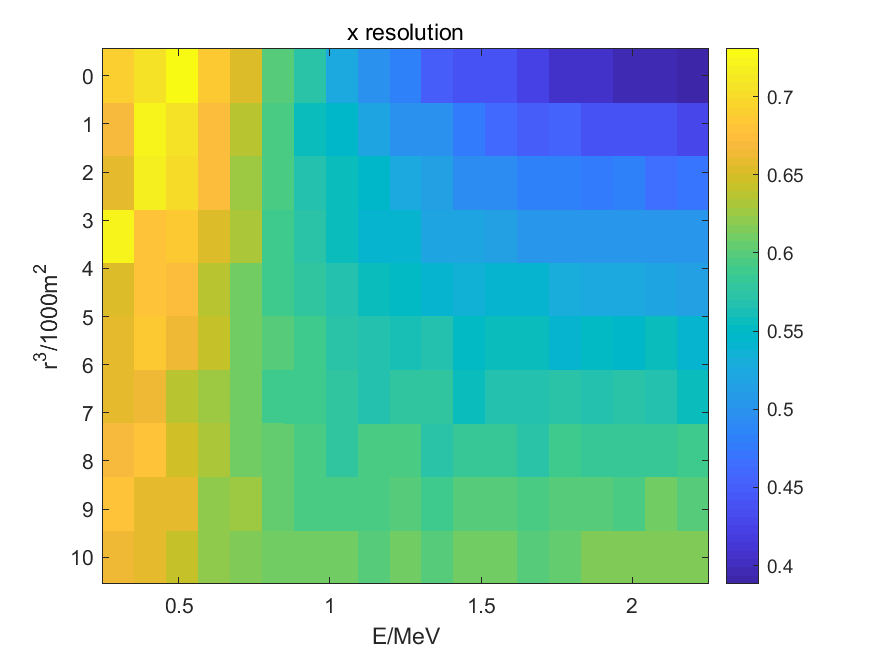
\includegraphics[width=2in]{./figure/x_res.png}
%\caption{fig1}
\end{minipage}%
}%
\subfigure[pic2.]{
\begin{minipage}[t]{0.5\linewidth}
\centering
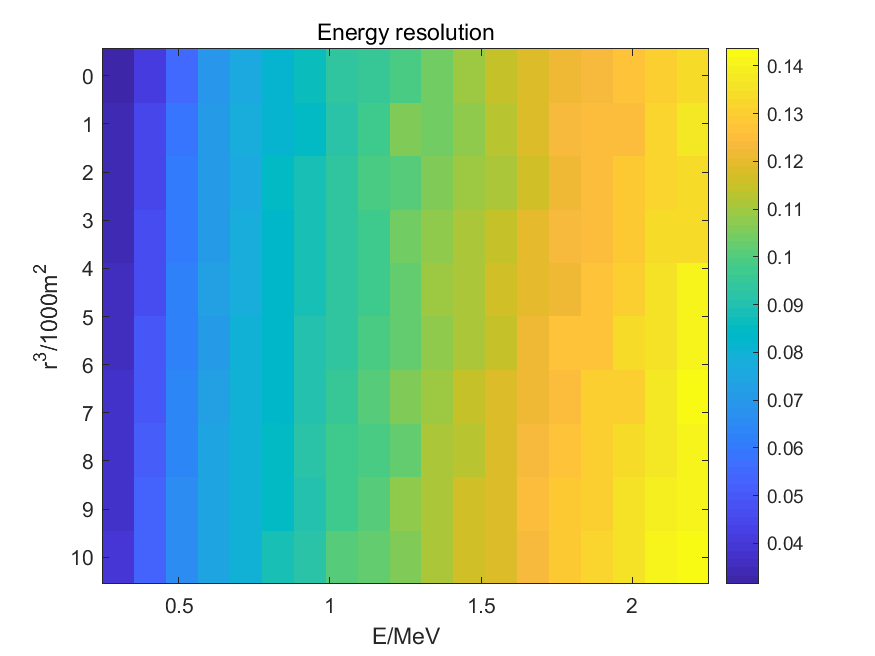
\includegraphics[width=2in]{./figure/E_res.png}
%\caption{fig2}
\end{minipage}%
}%


\subfigure[pic3.]{
\begin{minipage}[t]{0.5\linewidth}
\centering
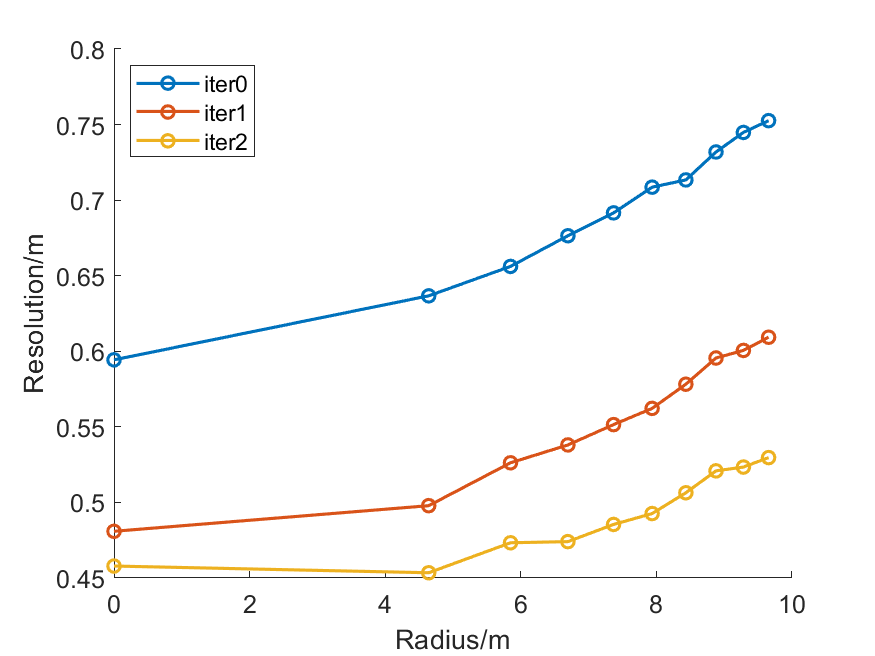
\includegraphics[width=2.2in]{./figure/iter1.png}
\label{fig:4.3}
%\caption{fig1}
\end{minipage}%
}%
\subfigure[pic4.]{
\begin{minipage}[t]{0.5\linewidth}
\centering
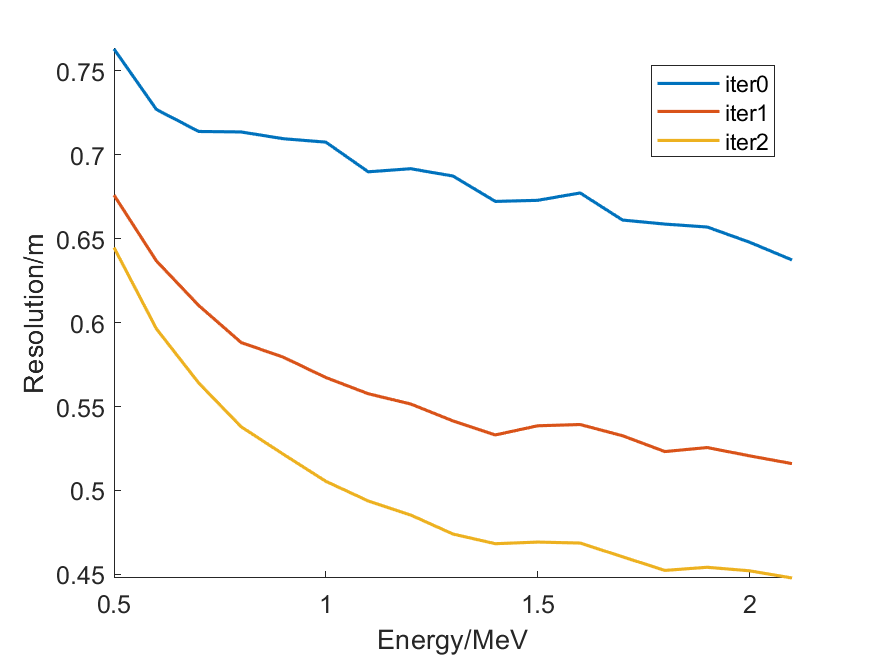
\includegraphics[width=2.2in]{./figure/iter2.png}
\label{fig:4.4}
%\caption{fig2}
\end{minipage}%
}%

\subfigure[pic5.]{
\begin{minipage}[t]{0.5\linewidth}
\centering
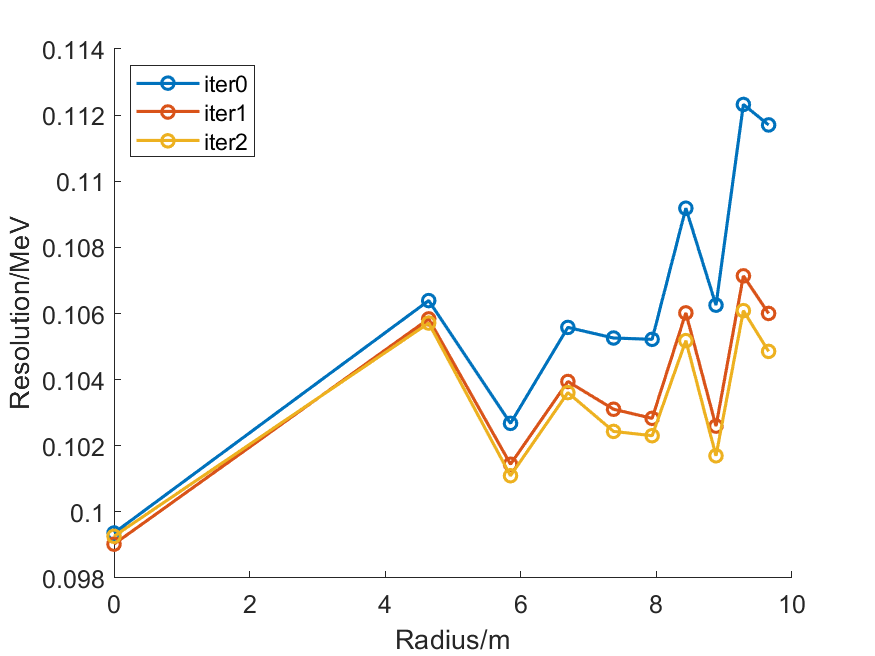
\includegraphics[width=2in]{./figure/iter3.png}
%\caption{fig2}
\end{minipage}
}%
\subfigure[pic6.]{
\begin{minipage}[t]{0.5\linewidth}
\centering
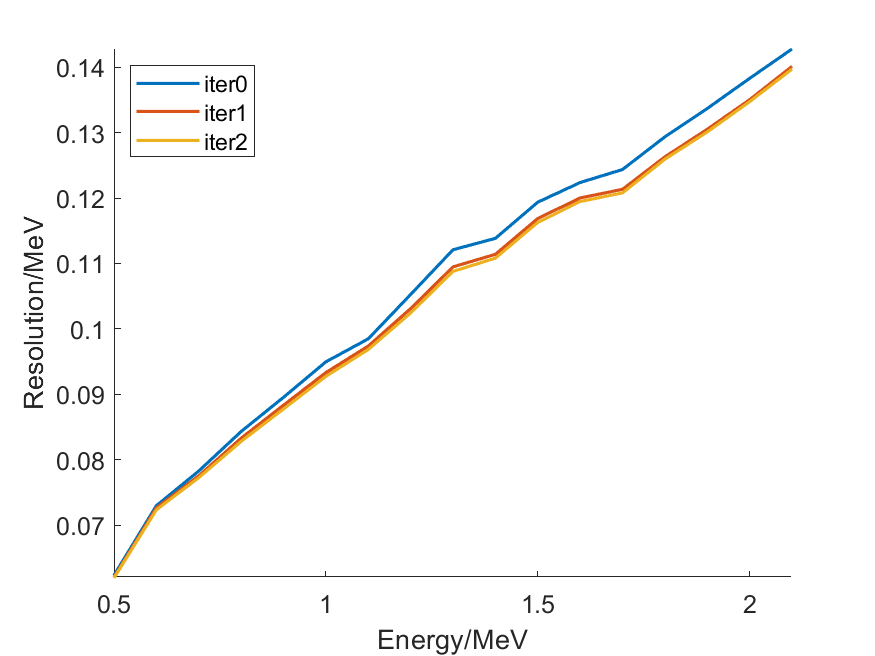
\includegraphics[width=2in]{./figure/iter4.png}
%\caption{fig2}
\end{minipage}
}%
\centering
\caption{ Reconstruction of energy and vertex}
\label{fig:4}
\end{figure}

\subsection{Process the data*} 
\subsubsection{Particle identification}
\par A cluster can applied to separate particles.
\subsubsection{Energy dependent time profile}
\par Decay time constant relative to energy can be plot by piece-wise function.

\section{Conclusion and Discussion}
\subsection{Achieved result}
\begin{itemize}
\item The $\tau_d$ can be reconstructed directly.
\item *$\tau_d$ is effective to PID
\item *Performance comparing to the situation with noise or Cherenkov. 
\end{itemize}

\subsection{What can be done in the future}
\begin{itemize}
\item Optics and geometry may be needed. 
\end{itemize}

\section{Appendix}
\subsection{Resolution derivation}
\subsection{Initial guess}
\end{document}
